\documentclass[12pt]{article}

\usepackage{amsmath, mathtools}
\usepackage{amsfonts}
\usepackage{amssymb}
\usepackage{graphicx}
\usepackage{colortbl}
\usepackage{xr}
\usepackage{hyperref}
\usepackage{longtable}
\usepackage{xfrac}
\usepackage{tabularx}
\usepackage{float}
\usepackage{siunitx}
\usepackage{booktabs}
\usepackage{caption}
\usepackage{pdflscape}
\usepackage{afterpage}

%\usepackage{refcheck}

\hypersetup{
    bookmarks=true,         % show bookmarks bar?
      colorlinks=true,       % false: boxed links; true: colored links
    linkcolor=red,          % color of internal links (change box color with linkbordercolor)
    citecolor=green,        % color of links to bibliography
    filecolor=magenta,      % color of file links
    urlcolor=cyan           % color of external links
}

%% Comments

\usepackage{color}

\newif\ifcomments\commentstrue

\ifcomments
\newcommand{\authornote}[3]{\textcolor{#1}{[#3 ---#2]}}
\newcommand{\todo}[1]{\textcolor{red}{[TODO: #1]}}
\else
\newcommand{\authornote}[3]{}
\newcommand{\todo}[1]{}
\fi

\newcommand{\wss}[1]{\authornote{blue}{SS}{#1}}
\newcommand{\an}[1]{\authornote{magenta}{Author}{#1}}


% For easy change of table widths
\newcommand{\colZwidth}{1.0\textwidth}
\newcommand{\colAwidth}{0.13\textwidth}
\newcommand{\colBwidth}{0.82\textwidth}
\newcommand{\colCwidth}{0.1\textwidth}
\newcommand{\colDwidth}{0.05\textwidth}
\newcommand{\colEwidth}{0.8\textwidth}
\newcommand{\colFwidth}{0.17\textwidth}
\newcommand{\colGwidth}{0.5\textwidth}
\newcommand{\colHwidth}{0.28\textwidth}

% Used so that cross-references have a meaningful prefix
\newcounter{defnum} %Definition Number
\newcommand{\dthedefnum}{GD\thedefnum}
\newcommand{\dref}[1]{GD\ref{#1}}
\newcounter{datadefnum} %Datadefinition Number
\newcommand{\ddthedatadefnum}{DD\thedatadefnum}
\newcommand{\ddref}[1]{DD\ref{#1}}
\newcounter{theorynum} %Theory Number
\newcommand{\tthetheorynum}{T\thetheorynum}
\newcommand{\tref}[1]{T\ref{#1}}
\newcounter{tablenum} %Table Number
\newcommand{\tbthetablenum}{T\thetablenum}
\newcommand{\tbref}[1]{TB\ref{#1}}
\newcounter{assumpnum} %Assumption Number
\newcommand{\atheassumpnum}{P\theassumpnum}
\newcommand{\aref}[1]{A\ref{#1}}
\newcounter{goalnum} %Goal Number
\newcommand{\gthegoalnum}{P\thegoalnum}
\newcommand{\gsref}[1]{GS\ref{#1}}
\newcounter{instnum} %Instance Number
\newcommand{\itheinstnum}{IM\theinstnum}
\newcommand{\iref}[1]{IM\ref{#1}}
\newcounter{reqnum} %Requirement Number
\newcommand{\rthereqnum}{P\thereqnum}
\newcommand{\rref}[1]{R\ref{#1}}
\newcounter{lcnum} %Likely change number
\newcommand{\lthelcnum}{LC\thelcnum}
\newcommand{\lcref}[1]{LC\ref{#1}}

\newcommand{\progname}{SpectrumImageAnalysisPy} % PUT YOUR PROGRAM NAME HERE

\usepackage{fullpage}

\begin{document}
\bibliographystyle{ieeetr}
\title{SpectrumImageAnalysisPy} 
\author{Isobel Bicket}
\date{\today}
	
\maketitle

~\newpage

\pagenumbering{roman}


\section{Revision History}

\begin{tabularx}{\textwidth}{p{4cm}p{2cm}X}
	\toprule {\bf Date} & {\bf Version} & {\bf Notes}\\
	\midrule
	\today & 1.0 & First draft\\
	\bottomrule
\end{tabularx}

~\newpage

\tableofcontents

\section{Reference Material}

This section records information for easy reference.

\subsection{Table of Units}

Throughout this document the system of units standard to the field of electron microscopy is used
as the unit system, for consistency with relevant literature and practices. For each unit, the symbol is given followed by a
description of the quantity described by the symbol and the unit name.
~\newline

\renewcommand{\arraystretch}{1.2}
%\begin{table}[ht]
  \noindent \begin{tabular}{l l l} 
    \toprule		
    \textbf{symbol} & \textbf{quantity} & \textbf{unit name}\\
    \midrule 
    \si{\nano\metre} & length & nanometre\\
    \si{\electronvolt} & energy	& electron volt\\
    \bottomrule
  \end{tabular}
  %	\caption{Provide a caption}
%\end{table}

\subsection{Table of Symbols}

The table that follows summarizes the symbols used in this document along with
their units. The symbols are listed in alphabetical order.

\renewcommand{\arraystretch}{1.2}
%\noindent \begin{tabularx}{1.0\textwidth}{l l X}
\noindent \begin{longtable*}{l l p{12cm}} \toprule
\textbf{symbol} & \textbf{unit} & \textbf{description}\\
\midrule 
$I$ &  & Intensity\\
$$ &  & \\ 
\bottomrule
\end{longtable*}

\subsection{Abbreviations and Acronyms}

\renewcommand{\arraystretch}{1.2}
\begin{tabular}{l l} 
  \toprule		
  \textbf{symbol} & \textbf{description}\\
  \midrule 
  3D & Three-dimensional\\
  A & Assumption\\
  CCD & Charge-Coupled Device\\
  CL & Cathodoluminescence Spectroscopy\\
  DD & Data Definition\\
  EELS & Electron Energy Loss\\
  EELS & Electron Energy Loss Spectroscopy\\
  GD & General Definition\\
  GS & Goal Statement\\
  IM & Instance Model\\
  LC & Likely Change\\
  PS & Physical System Description\\
  PSF & Point Spread Function\\
  R & Requirement\\
  SI & Spectrum Image\\
  SRS & Software Requirements Specification\\
  STEM & Scanning Transmission Electron Microscope\\
  SEM & Scanning Electron Microscope\\
  \progname{} & \wss{put your program name here}\\
  T & Theoretical Model\\
  \bottomrule
\end{tabular}\\

\wss{Add any other abbreviations or acronyms that you add}

\newpage
\pagenumbering{arabic}

\section{Introduction}

\wss{This SRS template is based on SmithAndLai2005, SmithEtAl2007.  It
  will get you started, but you will have to make changes.  Any changes to
  section headings should be approved by the instructor, since that implies a
  deviation from the template.  Although the bits shown below do not include
  type information, you may need to add this information for your problem.}

\wss{Feel free to change the appearance of the report by modifying the LaTeX
  commands.}

\wss{If you are documenting a family of models, you can start from this same
  template, but you will have to add a section for variabilities.  For program
  families you should look at \cite{Smith2006, SmithMcCutchanAndCarette2017}.
  You should be able to do one document that captures the commonality analysis
  and the requirements.}

\subsection{Purpose of Document}

This document details the requirements of the software \progname{}.

\subsection{Scope of Requirements} 
The scope of the requirements for the software \progname{} is limited to the import; removal of instrumentation artifacts; visualization and navigation through; and the export of EELS and CL spectrum imaging data.

\subsection{Characteristics of Intended Reader} 
The reader of this document should have an understanding of spectrum imaging techniques, particularly EELS and the data processing methods used to remove effects of the acquisition system from the data acquired. A basic knowledge of convolution theory will be helpful to the reader and an understanding of the characteristics of 3D datasets. The reader should understand EELS and CL, as relevant to the sections of the document.

\subsection{Organization of Document}

The document follows the organizational scheme laid out by Smith \textit{et al} \cite{SmithAndLai2005, smith_requirements_2007}.

\section{General System Description}

This section identifies the interfaces between the system and its environment,
describes the user characteristics and lists the system constraints.

\subsection{System Context}

Use of the software \progname{} infers the following responsibilities on the part of the user, and confers the following responsibilities from the program.

\begin{itemize}
	\item User Responsibilities:
	\begin{itemize}
		\item Provide the correct input data to the program;
		\item Be capable of interacting with the software via a mouse and keyboard;
		\item Have the necessary dependencies for the program installed;
		\item Possess sufficient knowledge on what processing steps need to be performed and be able to judge that the quality of the output data is sufficient for the application, or change the processing steps performed;
	\end{itemize}
	\item \progname{} Responsibilities:
	\begin{itemize}
		\item Read inputs (either files or data arrays) and check the inputs for the correct data type and size
		\item Display the data and graphical user interface for the user to interact with
		\item Respond to user commands as appropriate, including visualization and data processing commands
		\item Export data in the correct file format(s)
	\end{itemize}
\end{itemize}

\subsection{User Characteristics} \label{SecUserCharacteristics}

The end user of \progname{} should be familiar with the concept of a spectrum
image and an understanding of what the data represents and the appropriate
actions needed to process spectrum images and extract useful information. A basic familiarity with programming is expected. An
understanding of the spectro-microscopy technique (CL or EELS) used to generate the data will
be beneficial, but is not strictly required. 

\subsection{System Constraints}

The software must be able to read .dm3 files for EELS data import, and .h5 files for CL data import to be able to interface with output from the data acquisition software.

\section{Specific System Description}

This section first presents the problem description, which gives a high-level
view of the problem to be solved.  This is followed by the solution characteristics
specification, which presents the assumptions, theories, definitions and finally
the instance models.  \wss{Add any project specific details that are relevant
  for the section overview.}

\subsection{Problem Description} \label{Sec_pd}

\progname{} is a software to allow users to import, process, navigate, and export spectrum image data. 

\subsubsection{Terminology and  Definitions}

This subsection provides a list of terms that are used in the subsequent
sections and their meaning, with the purpose of reducing ambiguity and making it
easier to correctly understand the requirements:

\begin{itemize}
	\item Charge-Coupled Device: the camera used in the spectrometer to collect signal and output to the microscope acquisition software
	\item Spectrum Image
	\item Point Spread Function (PSF)
	\item Sample
\end{itemize}

\subsubsection{Physical System Description}

The physical system of \progname{}, as shown in Figure~?,
includes the following elements:

\begin{itemize}

	\item[PS1:] Sample under study.
	\item[PS2:] STEM equipped with EEL spectrometer.
	\an{Find an image/schematic of Titan}
	\item[PS3:] SEM or STEM equipped with CL collection system.
	\an{Find an image/schematic of SEM-CL system}

%\item[PS1:] Three dimensional dataset, including two spatial dimensions and one spectral dimension (eg, EELS: energy loss in \si{\electronvolt}, CL: wavelength in \si{\nano\metre}). The sample under study is represented in projection in the two spatial dimensions, while the third dimension represents the response of the sample to an external stimulus; for both EELS and CL, the external stimulus is a beam of fast electrons.
%
%\item[PS2:] A point spread function (PSF) (optional for EELS, not required for CL) representing the response of the instrument used to probe the sample. The experimental data collected can often be considered as a convolution of the ``real'' spectral response of the sample with the PSF. The PSF is a one dimensional spectrum.

\end{itemize}

%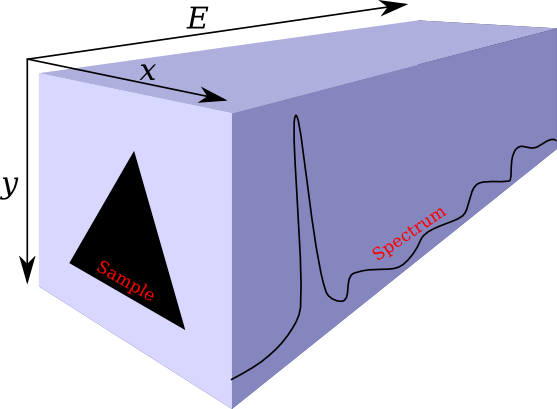
\includegraphics[]{SpectrumImageSchematic.png}


\wss{A figure here may make sense for most SRS documents}

% \begin{figure}[h!]
% \begin{center}
% %\rotatebox{-90}
% {
%  \includegraphics[width=0.5\textwidth]{<FigureName>}
% }
% \caption{\label{<Label>} <Caption>}
% \end{center}
% \end{figure}

\subsubsection{Goal Statements}

\noindent Given the \wss{inputs}, the goal statements are:

\begin{itemize}

	\item[GS\refstepcounter{goalnum}\thegoalnum \label{G_ImportDisplay}:] Import a 3D dataset and display it such that the user can interact with it and navigate all three dimensions
	\item[GS\refstepcounter{goalnum}\thegoalnum \label{G_Processing}:] Provide processing options including: normalization and deconvolution for EELS SI; normalization and background subtraction for a CL SI
	\item[GS\refstepcounter{goalnum}\thegoalnum \label{G_Extraction}:] Extract slices from the dataset as desired by the user and communicated through the user interface, export these as desired by the user

\end{itemize}

\subsection{Solution Characteristics Specification}

The instance models that govern \progname{} are presented in
Subsection~\ref{sec_instance}.  The information to understand the meaning of the
instance models and their derivation is also presented, so that the instance
models can be verified.

\subsubsection{Assumptions}

This section simplifies the original problem and helps in developing the
theoretical model by filling in the missing information for the physical
system. The numbers given in the square brackets refer to the theoretical model
[T], general definition [GD], data definition [DD], instance model [IM], or
likely change [LC], in which the respective assumption is used.

\begin{itemize}

	\item[A\refstepcounter{assumpnum}\theassumpnum \label{EELS_System_Response}:] The EELS data can be described as the convolution of the ``real'' spectrum of the sample with the response of the microscope and spectrometer system function. The microscope and spectrometer system typically causes broadening in the peaks of the ``real'' spectrum;
	
	\item[A\refstepcounter{assumpnum}\theassumpnum \label{EELS_PSF_variability}:] The same PSF is valid for all pixels in the EELS spectrum image;
	
	\item[A\refstepcounter{assumpnum}\theassumpnum \label{EELS_Intensity_Fluctuations}:] Fluctuations in the intensity of the EELS signal are due to changes in the beam current as collected by the spectrometer;
	
	\item[A\refstepcounter{assumpnum}\theassumpnum \label{CL_Background}:] A subtraction is sufficient remove the contributions of the dark signal and the substrate signal from the CL sample signal;
	
	\item[A\refstepcounter{assumpnum}\theassumpnum \label{CL_System_Response}:] The CL spectrometer wavelength sensitivity can be accurately modelled by experimental reference data.

\end{itemize}

\subsubsection{Theoretical Models}\label{sec_theoretical}

This section focuses on the general equations and laws that \progname{} is based
on.  \wss{Modify the examples below for your problem, and add additional models
  as appropriate.}

~\newline

\noindent
\begin{minipage}{\textwidth}
	\renewcommand*{\arraystretch}{1.5}
	\begin{tabular}{| p{\colAwidth} | p{\colBwidth}|}
		  \hline
		  \rowcolor[gray]{0.9}
		  Number& T\refstepcounter{theorynum}\thetheorynum \label{intensity}\\
		  \hline
		  Label&\bf Intensity \\
		  \hline
		  Equation& $\zeta(k) = g(k) S(k) + b(k) + N(k)$ \\
		  \hline
		  Description & The signal, $\zeta(k)$ (\tref{signal}), obtained from each pixel, $k$, on the CCD detector can be considered as a sum of several different contributions: 
		  \begin{itemize}
			\item the signal obtained from the microscope $S(k)$, which is multiplied by the gain factor $g(k)$ of the pixel; 
			\item the background signal of each pixel $b(k)$; 
			\item and the noise present at each pixel $N(k)$.
		  \end{itemize}\\
		  \hline
		  Source & \cite{zuo_electron_2000}
		           \\
		  % The above web link should be replaced with a proper citation to a publication
		  \hline
		  Ref.\ By & \\
		  \hline
	\end{tabular}
\end{minipage}\\

~\newline

\noindent
\begin{minipage}{\textwidth}
	\renewcommand*{\arraystretch}{1.5}
	\begin{tabular}{| p{\colAwidth} | p{\colBwidth}|}
		  \hline
		  \rowcolor[gray]{0.9}
		  Number& T\refstepcounter{theorynum}\thetheorynum \label{signal}\\
		  \hline
		  Label&\bf Signal \\
		  \hline
		  Equation& $S(k)=\int_{pixel}d\rho \lfloor \int f(\rho') h(\rho, \rho') d\rho' \rfloor$ \\
		  & $ S(k)=\sum_{k'} f(k') h(k, k')$\\
		  \hline
		  Description & The signal ($S(k)$) from the microscope, as read at one pixel on the CCD ($k$), is an integral over the area of one pixel. Inside the integral is the probability ($f(\rho')$) of an electron landing at position $\rho'$ on the detector given the interaction of the beam with the sample, multiplied by the probability ($h(\rho, \rho')$) of detecting an electron at location $\rho$ if the electron arrives at position $\rho'$ on the detector. The probability $h(\rho, \rho')$ of detecting an electron at one location after it hits the detector at another location is the point spread function (PSF: \ddref{PSF}).\\
		  & The second equation is the discretized version of the first. The signal $S(k)$ is the sum over all pixels $k'$ of the probability ($f(k')$) of an electron hitting pixel $k'$ multiplied by the probability ($h(k, k')$) of detecting an electron at $k$ after it hits pixel $k'$.\\
		  \hline
		  Source & \cite{zuo_electron_2000}\\
		  % The above web link should be replaced with a proper citation to a publication
		  \hline
		  Ref.\ By & \tref{intensity}\\
		  \hline
	\end{tabular}
\end{minipage}\\

~\newline

\subsubsection{General Definitions}\label{sec_gendef}

This section collects the laws and equations that will be used in deriving the
data definitions, which in turn are used to build the instance models.
\wss{Some projects may not have any content for this section, but the section
  heading should be kept.}  \wss{Modify the examples below for your problem, and
  add additional definitions as appropriate.}

~\newline

\noindent
\begin{minipage}{\textwidth}
	\renewcommand*{\arraystretch}{1.5}
	\begin{tabular}{| p{\colAwidth} | p{\colBwidth}|}
		\hline
		\rowcolor[gray]{0.9}
		Number& GD\refstepcounter{defnum}\thedefnum \label{grid}\\
		\hline
		Label & Scanning grid  \\
		\hline
		Units& \si{\nano\metre}\\
		\hline
		Equation& $P(x,y) = \{\langle x, y \rangle \in A^2 \mid x \in \{0..X\}, y \in \{0..Y\} \}$\\
		\hline
		Description & $P(x,y)$ is a set of position coordinates describing the possible locations of the beam in two spatial coordinates $(x, y)$ during a raster scan across the sample in a rectangular grid pattern across the area on the sample, $A^2$. The limits on $(x,y)$ are set by the operator on the instrument, ranging from 0 to the maximum $(X,Y)$.
		\\
		  \hline
		  Ref.\ By & \ddref{SI}\\
		  \hline
	\end{tabular}
\end{minipage}\\

\subsubsection{Data Definitions}\label{sec_datadef}

This section collects and defines all the data needed to build the instance
models. The dimension of each quantity is also given.  \wss{Modify the examples
  below for your problem, and add additional definitions as appropriate.}

~\newline

\noindent
\begin{minipage}{\textwidth}
	\renewcommand*{\arraystretch}{1.5}
	\begin{tabular}{| p{\colAwidth} | p{\colBwidth}|}
		\hline
		\rowcolor[gray]{0.9}
		Number& DD\refstepcounter{datadefnum}\thedatadefnum \label{Spectrum}\\
		\hline
		Label& \bf Spectrum\\
		\hline
		Symbol & $I(E)$\\
		\hline
		Units & Electron counts (EELS)\\
		& Photon counts (CL)\\
		& or arbitrary units (a.u.) for EELS or CL\\
		  \hline
		  Equation & $E = f(k)$\\
		  & $I(E) = \zeta(k=0..K)$\\
		  \hline
		  Description & Each pixel ($k$) on the spectrometer CCD has an energy loss (EELS) or wavelength (CL) value associated with it ($E$), obtained from the spectrometer acquisition settings (denoted here by $f(k)$), and a collected signal ($\zeta(k)$, \tref{signal}). The intensity of the spectrum ($I(E)$) is obtained from the collected signal over the whole CCD, from the 0th pixel to the final ($K$th) pixel.\\
		  \hline
		  Sources & \cite{egerton_introduction_2011} \\
		  \hline
		  Ref.\ By & \ddref{SI}\\
		  \hline
	\end{tabular}
\end{minipage}\\

~\newline

\noindent
\begin{minipage}{\textwidth}
\renewcommand*{\arraystretch}{1.5}
\begin{tabular}{| p{\colAwidth} | p{\colBwidth}|}
	\hline
	\rowcolor[gray]{0.9}
	Number& DD\refstepcounter{datadefnum}\thedatadefnum \label{SI}\\
	\hline
	Label& \bf Spectrum Image\\
	\hline
	Symbol &$I(x, y, E)$\\
	\hline
	Units & Electron counts (EELS)\\
	& Photons (CL)\\
	& or arbitrary units (a.u.) for EELS or CL\\
	\hline
	Equation& $I(x, y, E): \forall \langle x, y \rangle \in P(x,y), \exists I(E)$ \\
	\hline
	Description & $I(x, y, E)$ is a dataset composed of Spectra (\ddref{Spectrum}) collected by the spectrometer detector at each value of $P(x,y)$ (\dref{grid}).
	\\
	\hline
	Sources&~\cite{jeanguillaume_spectrum-image:_1989}  \\
	\hline
	Ref.\ By & \\
	\hline
\end{tabular}
\end{minipage}\\

~\newline

\noindent
\begin{minipage}{\textwidth}
	\renewcommand*{\arraystretch}{1.5}
	\begin{tabular}{| p{\colAwidth} | p{\colBwidth}|}
		\hline
		\rowcolor[gray]{0.9}
		Number& DD\refstepcounter{datadefnum}\thedatadefnum \label{PSF}\\
		\hline
		Label& \bf Point Spread Function\\
		\hline
		Symbol &$I_PSF(E)$\\
		\hline
		Units & Electron counts or arbitrary units (a.u.) (EELS)\\
		  \hline
		  Equation&$I(E) = \zeta(k={0..K}) = g(k) S'(k) + b(k) + N(k)$\\
		  \hline
		  Description & 
		               $I_PSF(E)$ is a reference spectrum ($I(E)$, \ddref{Spectrum}) representing the effect of the point spread function (see \tref{signal}) on the collected spectra in the spectrum image (\ddref{SI}). It is a spectrum collected, ideally, with no interaction with a sample; the variables in the equation are defined as in \tref{intensity}, with the exception of $S'(k)$, which is an example of $S(k)$ with no sample interaction with the beam.
		  \\
		  \hline
		  Sources&~\cite{zuo_electron_2000, jeanguillaume_spectrum-image:_1989, gloter_improving_2003}  \\
		  \hline
		  Ref.\ By & \iref{ewat}\\
		  \hline
	\end{tabular}
\end{minipage}\\

\subsubsection{Instance Models} \label{sec_instance}    

This section transforms the problem defined in Section~\ref{Sec_pd} into 
one which is expressed in mathematical terms. It uses concrete symbols defined 
in Section~\ref{sec_datadef} to replace the abstract symbols in the models 
identified in Sections~\ref{sec_theoretical} and~\ref{sec_gendef}.

The goals \wss{reference your goals} are solved by \wss{reference your instance
  models}.  \wss{other details, with cross-references where appropriate.}
\wss{Modify the examples below for your problem, and add additional models as
  appropriate.}

~\newline

%Instance Model 1

\noindent
\begin{minipage}{\textwidth}
	\renewcommand*{\arraystretch}{1.5}
	\begin{tabular}{| p{\colAwidth} | p{\colBwidth}|}
		  \hline
		  \rowcolor[gray]{0.9}
		  Number& IM\refstepcounter{instnum}\theinstnum \label{normalization}\\
		  \hline
		  Label& \bf Normalization to the integral\\
		  \hline
		  Input& $k_1$\\
		  & $k_2$\\
		  & $I(x,y,E_k)$\\
		  & The input is constrained such that $k_1 >= 0$, and $k_2 <= N$\\
		  \hline
		  Output& $I_{norm}(x,y,E_k)=\frac{I(x,y,E_k)}{\sum_{E_{k=k_1}}^{E_{k=k_2}} I(x,y,E_k)}$\\
		  \hline
		  Description&$I(x,y,E_k)$ is the 3D spectrum image, user input\\
		  &$k_1$: Index of beginning of spectrum range (spectrum axis), user input\\
		  &$k_2$: Index of end of spectrum range (spectrum axis), user input\\
		  &$K$: Last index along the spectral axis\\
		  &$x$: Pixel index along first spatial axis\\
		  &$y$: Pixel index along second spatial axis\\
		  &$I_{norm}(x,y,E_k)$: Spectrum image with each individual pixel normalized independently along the spectral axis\\
		  \hline
		  Sources&\\
		  \hline
		  Ref.\ By &\\
		  \hline
	\end{tabular}
\end{minipage}\\

~\newline

%Instance Model 2

\noindent
\begin{minipage}{\textwidth}
	\renewcommand*{\arraystretch}{1.5}
	\begin{tabular}{| p{\colAwidth} | p{\colBwidth}|}
		\hline
		\rowcolor[gray]{0.9}
		Number& IM\refstepcounter{instnum}\theinstnum \label{deconvolution}\\
		\hline
		Label& \bf Richardson-Lucy Deconvolution\\
		\hline
		Input& $I_PSF(E)$ is the point spread function of the instrument (see \ddref{PSF})\\
		& $I_{real}^0(x,y,E)$ is the initial guess for the ``real'' spectrum (\ddref{Spectrum})\\
		& $I_{measured}(x,y,E)$ is the measured spectrum, as obtained from the spectrometer software (\ddref{Spectrum})\\
		& $R$ is the number of iterations of the deconvolution algorithm applied to the spectrum \\
		\hline
		Equation & $I_{real (b)}^{c+1}(E)=I_{real (b)}^c(E)\sum_a{\frac{I_{PSF}(E)I_{measured}(E)}{\sum_d{I_{PSF}(E)I_{real (d)}^c(E)}}}, while\ c < R$\\
		\hline
		Output& $I_{deconvolved}(E_k)=I_{real (b)}^{R}(E)$\\
		\hline
		Description & The purpose of the RL deconvolution algorithm is to separate the effects of the spectrometer point spread function from the ``real'' signal of the sample. \textit{I.e.} In \tref{signal}, the signal is described as the convolution of the point spread function with the signal from the microscope.\\
		\hline
		Sources&~\cite{gloter_improving_2003, bellido_toward_2014} \ \\
		\hline
		Ref.\ By & \\
		\hline
	\end{tabular}
\end{minipage}\\

%~\newline

\subsubsection*{Derivation of ...}

\wss{May be necessary to include this subsection in some cases.}

\subsubsection{Data Constraints} \label{sec_DataConstraints}    

Tables~\ref{TblInputVar} and \ref{TblOutputVar} show the data constraints on the
input and output variables, respectively.  The column for physical constraints gives
the physical limitations on the range of values that can be taken by the
variable.  The column for software constraints restricts the range of inputs to
reasonable values.  The constraints are conservative, to give the user of the
model the flexibility to experiment with unusual situations.  The column of
typical values is intended to provide a feel for a common scenario.  The
uncertainty column provides an estimate of the confidence with which the
physical quantities can be measured.  This information would be part of the
input if one were performing an uncertainty quantification exercise.

The specification parameters in Table~\ref{TblInputVar} are listed in
Table~\ref{TblSpecParams}.

\begin{table}[!h]
	  \caption{Input Variables} \label{TblInputVar}
	  \renewcommand{\arraystretch}{1.2}
	\noindent \begin{longtable*}{l l l l c} 
		  \toprule
		  \textbf{Var} & \textbf{Physical Constraints} & \textbf{Software Constraints} &
		                             \textbf{Typical Value} & \textbf{Uncertainty}\\
		  \midrule 
		  && &
		  \\
		  \bottomrule
	\end{longtable*}
\end{table}

\noindent 
\begin{description}
\item[(*)] \wss{you might need to add some notes or clarifications}
\end{description}

\begin{table}[!h]
	\caption{Specification Parameter Values} \label{TblSpecParams}
	\renewcommand{\arraystretch}{1.2}
	\noindent \begin{longtable*}{l l} 
	  \toprule
	  \textbf{Var} & \textbf{Value} \\
	  \midrule 
	   & \\
	  \bottomrule
	\end{longtable*}
\end{table}

\begin{table}[!h]
	\caption{Output Variables} \label{TblOutputVar}
	\renewcommand{\arraystretch}{1.2}
	\noindent \begin{longtable*}{l l} 
	  \toprule
	  \textbf{Var} & \textbf{Physical Constraints} \\
	  \midrule 
	   & 
	  \\
	  \bottomrule
	\end{longtable*}
\end{table}

\subsubsection{Properties of a Correct Solution} \label{sec_CorrectSolution}

\noindent
A correct solution must be acceptable to a user experienced with EELS and/or CL data processing, as is relevant to the EELS/CL data being processed.

\section{Requirements}

This section provides the functional requirements, the business tasks that the
software is expected to complete, and the nonfunctional requirements, the
qualities that the software is expected to exhibit.

\subsection{Functional Requirements}

\noindent \begin{itemize}

\item[R\refstepcounter{reqnum}\thereqnum \label{R_Inputs}:] Accept and read the following as Spectrum Image inputs:

\begin{itemize}
	\item 3D data array
	\item File in format *.dm3 containing 3D data array
	\item File in format *.h5 containing 3D data array
\end{itemize}

\item[R\refstepcounter{reqnum}\thereqnum \label{R_Inputs}:] Accept and read the following as Spectrum inputs:

\begin{itemize}
	\item 1D data array
	\item File containing 1D data array in *.csv format
\end{itemize}

\item[R\refstepcounter{reqnum}\thereqnum \label{R_Inputs}:] Verify that the data input is of the correct dimensionality and composed of Real numbers

\item[R\refstepcounter{reqnum}\thereqnum \label{R_Inputs}:] Accept user input to select a spectral range and extract (x,y) slices averaged over the selected spectral range and display the (x,y) slice as an image. The software should also export this image to an image file, as desired by the user.

\item[R\refstepcounter{reqnum}\thereqnum \label{R_Inputs}:] Accept user input to define an area on an (x,y) image display and extract a spectrum averaged over selected pixels. The software should also export this spectrum as a *.csv file, as desired by the user.

\item[R\refstepcounter{reqnum}\thereqnum \label{R_Inputs}:] Given a 1D spectrum array and an integer number, the software should perform that number of deconvolution iterations on a 3D EELS dataset using the 1D spectrum array as a reference of the system response. The software should display the output of the deconvolution for navigation by the user. Output of the deconvolution algorithm will be validated by an expert user. 

\item[R\refstepcounter{reqnum}\thereqnum \label{R_Inputs}:] The software should be able to normalize a 3D spectrum image upon user command: either to an integrated portion of a chosen range along the spectral axis or to a single chosen channel.

\item[R\refstepcounter{reqnum}\thereqnum \label{R_OutputInputs}:] \wss{It isn't
    always required, but often echoing the inputs as part of the output is a
    good idea.}

\item[R\refstepcounter{reqnum}\thereqnum \label{R_Calculate}:] \wss{Calculation
    related requirements.}

\item[R\refstepcounter{reqnum}\thereqnum \label{R_VerifyOutput}:]
  \wss{Verification related requirements.}

\item[R\refstepcounter{reqnum}\thereqnum \label{R_Output}:] \wss{Output related
    requirements.}

\end{itemize}

\subsection{Nonfunctional Requirements}

\wss{List your nonfunctional requirements.  You may consider using a fit
  criterion to make them verifiable.}

\section{Likely Changes}    

\noindent \begin{itemize}

\item[LC\refstepcounter{lcnum}\thelcnum\label{LC_meaningfulLabel}:] \wss{Give
    the likely changes, with a reference to the related assumption (aref), as appropriate.}

\end{itemize}

\section{Traceability Matrices and Graphs}

The purpose of the traceability matrices is to provide easy references on what
has to be additionally modified if a certain component is changed.  Every time a
component is changed, the items in the column of that component that are marked
with an ``X'' may have to be modified as well.  Table~\ref{Table:trace} shows the
dependencies of theoretical models, general definitions, data definitions, and
instance models with each other. Table~\ref{Table:R_trace} shows the
dependencies of instance models, requirements, and data constraints on each
other. Table~\ref{Table:A_trace} shows the dependencies of theoretical models,
general definitions, data definitions, instance models, and likely changes on
the assumptions.

\wss{You will have to modify these tables for your problem.}

\afterpage{
\begin{landscape}
	\begin{table}[h!]
		\centering
		\begin{tabular}{|c|c|c|c|c|c|c|c|c|c|c|c|c|c|c|c|c|c|c|c|}
		\hline
			& \aref{A_OnlyThermalEnergy}& \aref{A_hcoeff}& \aref{A_mixed}& \aref{A_tpcm}& \aref{A_const_density}& \aref{A_const_C}& \aref{A_Newt_coil}& \aref{A_tcoil}& \aref{A_tlcoil}& \aref{A_Newt_pcm}& \aref{A_charge}& \aref{A_InitTemp}& \aref{A_OpRangePCM}& \aref{A_OpRange}& \aref{A_htank}& \aref{A_int_heat}& \aref{A_vpcm}& \aref{A_PCM_state}& \aref{A_Pressure} \\
		\hline
		\tref{T_COE}        & X& & & & & & & & & & & & & & & & & & \\ \hline
		\tref{T_SHE}        & & & & & & & & & & & & & & & & & & & \\ \hline
		\tref{T_LHE}        & & & & & & & & & & & & & & & & & & & \\ \hline
		\dref{NL}           & & X& & & & & & & & & & & & & & & & & \\ \hline
		\dref{ROCT}         & & & X& X& X& X& & & & & & & & & & & & & \\ \hline
		\ddref{FluxCoil}    & & & & & & & X& X& X& & & & & & & & & & \\ \hline
		\ddref{FluxPCM}     & & & X& X& & & & & & X& & & & & & & & & \\ \hline
		\ddref{D_HOF}       & & & & & & & & & & & & & & & & & & & \\ \hline
		\ddref{D_MF}        & & & & & & & & & & & & & & & & & & & \\ \hline
		\iref{ewat}         & & & & & & & & & & & X& X& & X& X& X& & & X \\ \hline
		\iref{epcm}         & & & & & & & & & & & & X& X& & & X& X& X& \\ \hline
		\iref{I_HWAT}       & & & & & & & & & & & & & & X& & & & & X \\ \hline
		\iref{I_HPCM}       & & & & & & & & & & & & & X& & & & & X & \\ \hline
		\lcref{LC_tpcm}     & & & & X& & & & & & & & & & & & & & & \\ \hline
		\lcref{LC_tcoil}    & & & & & & & & X& & & & & & & & & & & \\ \hline
		\lcref{LC_tlcoil}   & & & & & & & & & X& & & & & & & & & & \\ \hline
		\lcref{LC_charge}   & & & & & & & & & & & X& & & & & & & & \\ \hline
		\lcref{LC_InitTemp} & & & & & & & & & & & & X& & & & & & & \\ \hline
		\lcref{LC_htank}    & & & & & & & & & & & & & & & X& & & & \\
		\hline
		\end{tabular}
		\caption{Traceability Matrix Showing the Connections Between Assumptions and Other Items}
		\label{Table:A_trace}
	\end{table}
\end{landscape}
}

\begin{table}[h!]
\centering
\begin{tabular}{|c|c|c|c|c|c|c|c|c|c|c|c|c|c|c|c|c|c|c|c|c|c|c|c|}
\hline        
	& \tref{T_COE}& \tref{T_SHE}& \tref{T_LHE}& \dref{NL}& \dref{ROCT} & \ddref{FluxCoil}& \ddref{FluxPCM} & \ddref{D_HOF}& \ddref{D_MF}& \iref{ewat}& \iref{epcm}& \iref{I_HWAT}& \iref{I_HPCM} \\
\hline
\tref{T_COE}     & & & & & & & & & & & & & \\ \hline
\tref{T_SHE}     & & & X& & & & & & & & & & \\ \hline
\tref{T_LHE}     & & & & & & & & & & & & & \\ \hline
\dref{NL}        & & & & & & & & & & & & & \\ \hline
\dref{ROCT}      & X& & & & & & & & & & & & \\ \hline
\ddref{FluxCoil} & & & & X& & & & & & & & & \\ \hline
\ddref{FluxPCM}  & & & & X& & & & & & & & & \\ \hline
\ddref{D_HOF}    & & & & & & & & & & & & & \\ \hline
\ddref{D_MF}     & & & & & & & & X& & & & & \\ \hline
\iref{ewat}      & & & & & X& X& X& & & & X& & \\ \hline
\iref{epcm}      & & & & & X& & X& & X& X& & & X \\ \hline
\iref{I_HWAT}    & & X& & & & & & & & & & & \\ \hline
\iref{I_HPCM}    & & X& X& & & & X& X& X& & X& & \\
\hline
\end{tabular}
\caption{Traceability Matrix Showing the Connections Between Items of Different Sections}
\label{Table:trace}
\end{table}

\begin{table}[h!]
\centering
\begin{tabular}{|c|c|c|c|c|c|c|c|}
\hline
	& \iref{ewat}& \iref{epcm}& \iref{I_HWAT}& \iref{I_HPCM}& \ref{sec_DataConstraints}& \rref{R_RawInputs}& \rref{R_MassInputs} \\
\hline
\iref{ewat}            & & X& & & & X& X \\ \hline
\iref{epcm}            & X& & & X& & X& X \\ \hline
\iref{I_HWAT}          & & & & & & X& X \\ \hline
\iref{I_HPCM}          & & X& & & & X& X \\ \hline
\rref{R_RawInputs}     & & & & & & & \\ \hline
\rref{R_MassInputs}    & & & & & & X& \\ \hline
\rref{R_CheckInputs}   & & & & & X& & \\ \hline
\rref{R_OutputInputs}  & X& X& & & & X& X \\ \hline
\rref{R_TempWater}     & X& & & & & & \\ \hline 
\rref{R_TempPCM}       & & X& & & & & \\ \hline
\rref{R_EnergyWater}   & & & X& & & & \\ \hline
\rref{R_EnergyPCM}     & & & & X& & & \\ \hline
\rref{R_VerifyOutput}  & & & X& X& & & \\ \hline
\rref{R_timeMeltBegin} & & X& & & & & \\ \hline
\rref{R_timeMeltEnd}   & & X& & & & & \\ 
\hline
\end{tabular}
\caption{Traceability Matrix Showing the Connections Between Requirements and Instance Models}
\label{Table:R_trace}
\end{table}

The purpose of the traceability graphs is also to provide easy references on
what has to be additionally modified if a certain component is changed.  The
arrows in the graphs represent dependencies. The component at the tail of an
arrow is depended on by the component at the head of that arrow. Therefore, if a
component is changed, the components that it points to should also be
changed. Figure~\ref{Fig_ATrace} shows the dependencies of theoretical models,
general definitions, data definitions, instance models, likely changes, and
assumptions on each other. Figure~\ref{Fig_RTrace} shows the dependencies of
instance models, requirements, and data constraints on each other.

% \begin{figure}[h!]
% 	\begin{center}
% 		%\rotatebox{-90}
% 		{
% 			\includegraphics[width=\textwidth]{ATrace.png}
% 		}
% 		\caption{\label{Fig_ATrace} Traceability Matrix Showing the Connections Between Items of Different Sections}
% 	\end{center}
% \end{figure}


% \begin{figure}[h!]
% 	\begin{center}
% 		%\rotatebox{-90}
% 		{
% 			\includegraphics[width=0.7\textwidth]{RTrace.png}
% 		}
% 		\caption{\label{Fig_RTrace} Traceability Matrix Showing the Connections Between Requirements, Instance Models, and Data Constraints}
% 	\end{center}
% \end{figure}

\newpage

\bibliography {SRS}

\newpage

\section{Appendix}

\wss{Your report may require an appendix.  For instance, this is a good point to
show the values of the symbolic parameters introduced in the report.}

\subsection{Symbolic Parameters}

\wss{The definition of the requirements will likely call for SYMBOLIC\_CONSTANTS.
Their values are defined in this section for easy maintenance.}

\end{document}